
% Let us assume that:
% \begin{align}
% \label{tri/1/eq:tri_basic}
% \vec{A} = \myvec{p\\q}, \vec{B} = \myvec{0\\0}, \vec{C} = \myvec{a\\0}, \vec{D} = \myvec{p\\0}
% \end{align}
% %
% Then
% \begin{align}
% \label{tri/1/eq:c_tricoord}
% AB &= \norm{\vec{A}-\vec{B}}^2 = \norm{\vec{A}}^2  = c^2 \quad \because \vec{B} = \vec{0}
% \\
% \label{tri/1/eq:a_tricoord}
% BC &= \norm{\vec{C}-\vec{B}}^2 = \norm{\vec{C}}^2  = a^2
% \\
% AC &= \norm{\vec{A}-\vec{C}}^2 =    b^2
% \label{tri/1/eq:b_tricoord}
% \end{align}
% %
% From \eqref{tri/1/eq:b_tricoord},
The vertex  $\vec{A}$ can  be expressed  in {\em polar coordinate form} as
%\label{tri/1/prob:tri_polar}
\begin{align}
\vec{A} = c\myvec{\cos B \\  \sin B} 
\end{align}
From $\triangle ABC$,we use the law of cosines: 
\begin{align}
% b^2 = a^2 + c^2 - 2ac \cos B
% \\
\cos B &= \frac{a^2+c^2-b^2}{2ac}
% \\
%  &= \frac{27}{48}
\\
&= 0.5625
\\
\implies {B} &= 55.771 \degree
\end{align}
Thus, 
\begin{align}
\vec{A} = 6\myvec{\cos 55.771 \\ \sin 55.771 }
\\
\vec{A} = \myvec{3.375\\4.960}, 
\vec{B} = \myvec{0\\0}, \vec{C} = \myvec{4\\0}.
\end{align}
which are plotted in Fig. \ref{tri/1/fig:tri_sss_triangle}	
\begin{figure}[!ht]
\centering
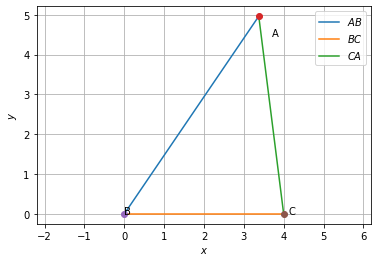
\includegraphics[width=\columnwidth]{solutions/triangle/1/download.png}
\caption{ $\triangle ABC$}
\label{tri/1/fig:tri_sss_triangle}	
\end{figure}
